La Transmission Control Protocol (TCP) est un protocole de transport en réseau qui est fiable et en mode connecté.
Le TCP fonctionne en trois phases disctinctes :
\begin{enumerate}
    \item Établissement de la connexion
    \item Transfère des données
    \item Fin de connexion
\end{enumerate}
\begin{figure}[h]
    \centering
    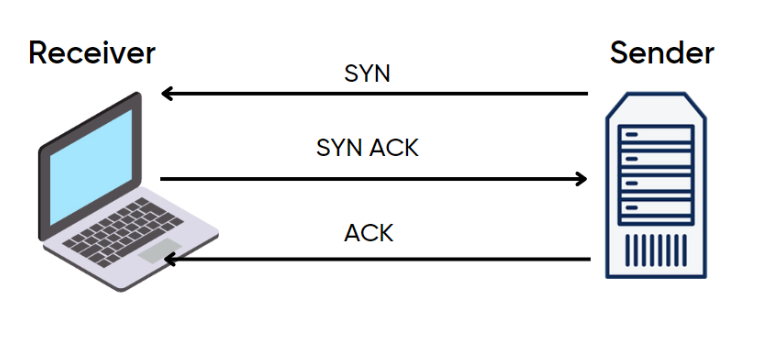
\includegraphics[width=100mm, height=50mm]{images/TCP.png}
    \caption{Schéma explicatif TCP}
    \label{img:mesh13}
\end{figure}
\newpage